\section{Analyse}
\subsection{Domänenmodell}
Das folgende Domänenmodell zeigt eine grobe Übersicht der Ausgangslage,
der identifizierten Objekte und Tätigkeiten der Benutzer.

Das Domänenmodell wurde aus dieser Liste von Konzeptklassen abgeleitet:

\begin{longtabu} to \textwidth { | l | X[l] | }
\hline
\textbf{Konzeptklassen} & \textbf{Beispiele} \\\hline
\endhead
Container/Hauptziel         & Trip, Tour                                               \\\hline
Interessante Orte/Wege     & Route, Point of Interest                                \\\hline
Orte                       & City, Country, TouristLocation                           \\\hline
Physische Akteure          & TouristAgency, Tourist                                   \\\hline
Ergebnisse einer Tour      & Photo, TourSummary, TourProgress, SocialMediaPost, Rating \\\hline
Tourüberwachung           & TourProgress, TourTracker                                \\\hline
Vermittlung von Information & Map, Marker                                              \\\hline
\end{longtabu}

\begin{figure}
  \centering
  \includegraphics{domain_model}
  \caption{Domänenmodell}
\end{figure}

\begin{longtabu} to \textwidth { | l | X[l] | }
\hline
\textbf{Objekte} & \textbf{Beschreibung} \\\hline
\endhead

Tourist & Dies ist die Hauptakteurin, der Hauptakteur und Benutzer_in der App. Er wählt eine \textbf{Tour} aus, läuft die \textbf{Route} ab, bringt seine Position durch eine \textbf{Map} in Erfahrung, überprüft seinen Fortschritt (\textbf{TourProgress}) und die Zusammenfassung \textbf{TourSummary}. \\\hline
TouristLocation & Repräsentiert die aktuelle Position der \textbf{Touristin}. \\\hline
TouristAgency & Reisebüros und Tourismusorganisationen erfassen Inhalt (d.h.: \textbf{Touren}, \textbf{Routen} und \textbf{Point of Interests}).\\\hline
Trip & Eine \textbf{Touristin} macht eine Reise (\textbf{Trip}) und hat dort je nach Ort und Stadt mehrere verschiedene \textbf{Touren} zur Auswahl.\\\hline
Tour & Eine \textbf{Tour} ist eine Sammlung von \textbf{Point of Interest}s in einer bestimmten Stadt \textbf{City}, die über eine bestimmte \textbf{Route} miteinander verbunden sind.\\\hline
TourRating & Der \textbf{Tourist} hat die Möglichkeit die \textbf{Tour} am Ende zu Bewertung und einen Kommentar zu hinterlassen. Die \textbf{TouristAgencies} haben Zugang zu diesen Bewertungen.\\\hline
TourProgress & Die \textbf{Touristin} kann aktuelle Metriken während der \textbf{Tour} überprüfen. \\\hline
TourSummary & Am Ende einer \textbf{Tour}, nachdem alle \textbf{Points of Interest} besucht wurden, wird dem \textbf{Touristen} eine Zusammenfassung/Statistik \textbf{TourSummary} über seine absolvierte \textbf{Route}, Anzahl Schritte, Distanz usw\ldots{} angezeigt.\\\hline
Route & Eine \textbf{Route} stellt eine Verbindung von mehreren \textbf{Point of Interests} dar. Eine \textbf{Route} kann mit verschiedenen \textbf{Verkehrsmitteln} absolviert werden.\\\hline
Map & Die Karte zeigt der \textbf{Touristin} mithilfe des \textbf{LocationMarkers} an. \\\hline
LocationMarker & Visuallisiert eine Position auf der Karte \textbf{Map}. \\\hline
City & Enthält mehere \textbf{Trips}. \\\hline
Country & Enthählt mehere Städte (\textbf{City}).\\\hline
Point of Interest & \textbf{Point of Interest} sind geographische Punkte, die eine Sehenswürdigkeit oder sonstige spezielle Eigenschaften bieten. Sie werden von einer \textbf{Route} verbunden. Der \textbf{Tourist} muss beim Absolvieren einer \textbf{Tour} an jedem \textbf{Point of Interest} vorbeikommen und ein \textbf{Foto} schiessen.\\\hline
Means of Transportation & Verschiedene \textbf{Verkehrsmittel} z.B.: Uber, ÖV, Auto, Velo, zu Fuss usw\ldots{}\\\hline
Foto & An jedem \textbf{Point of Interest} schiesst der Tourist mit seiner \textbf{Mobile App} ein \textbf{Foto} des Ortes oder der Sehenswürdigkeit. Wird das \textbf{Foto} akzeptiert, dann gilt der \textbf{Point of Interest} als besucht.\\\hline
SocialMediaPost & Die \textbf{Touristin} hat am Ende einer \textbf{Tour} die Möglichkeit, die Zusammenfassung (\textbf{TourSummary}) inklusive \textbf{Fotos} auf Social-Media-Kanälen zu teilen. \\\hline
\end{longtabu}

\newpage
\subsection{Anwendungsfälle}
\subsubsection{UC 1: Tour auswählen und starten (Priorität 1)}\label{uc-1-user-wuxe4hlt-tour-aus-und-startet-die-tour-priorituxe4t-1}
\subsubsubsection{Primärer Akteur}\label{primuxe4rer-akteur}
Tourist\_in


\subsubsubsection{Stakeholders und Interessen}\label{stakeholders-und-interessen}
\begin{itemize}
  \item Tourist\_in: Will mit einfachen Schritten eine passende Tour finden und starten.
  \item Premium Tour Anbieter\_in: Will seine Tour prominent plaziert haben um öfters ausgewählt zu werden.
\end{itemize}


\subsubsubsection{Vorbedingungen}\label{vorbedingungen}
\begin{itemize}
  \item Tourist\_in ist angemeldet.
  \item Touren sind auf Server erfasst.
\end{itemize}


\subsubsubsection{Erfolgsgarantie}\label{erfolgsgarantie}
Tourist\_in findet eine ansprechende Tour und kann diese starten.


\subsubsubsection{Standardablauf}\label{standardablauf}
\begin{enumerate}
  \item Tourist\_in öffnet app.
  \item Tourist\_in klickt auf neue Tour starten.
  \item System zeigt Auswahl von Touren an.
  \item Tourist\_in öffnet Filter.
  \item Tourist\_in setzt Filter um gewünschte Tour zu finden.
  \item Tourist\_in klickt auf Tour.
  \item System startet Tour.
  \item Tourist\_in begibt sich zum Startpunkt der Tour.
\end{enumerate}


\subsubsubsection{Erweiterungen}\label{erweiterungen}
\begin{enumerate}
  \setcounter{enumi}{3}
  \item
    \begin{enumerate}
      \item Auswahl ist abhängig von gerade populären oder von Premium Anbietern beworbenen Touren.
    \end{enumerate}

  \setcounter{enumi}{6}
  \item
    \begin{enumerate}
      \item App zeigt Detailvorschau an.
      \item Tourist\_in klickt auf Tour starten oder schliessen.
    \end{enumerate}

  \setcounter{enumi}{8}
  \item
    \begin{enumerate}
      \item Die App zeigt der Touristin verschiedene Möglichkeiten an, wie sie zum Startpunkt kommt.
    \end{enumerate}
\end{enumerate}


\subsubsubsection{Spezielle Anforderungen}\label{spezielle-anforderungen}
\begin{itemize}
  \item Filtern der Touren muss flüssig reagieren, Resultate werden sofort angezeigt.
\end{itemize}


\subsubsubsection{Auftrittshäufigkeit}\label{auftrittshuxe4ufigkeit}
Einmal pro Tour.


\subsubsection{UC 2: Route ablaufen und aktuellen Standort auf Karte betrachten (Priorität 2)}\label{uc-2-user-luxe4uft-route-ab-und-sieht-seine-aktuellen-standort-auf-einer-karte-priorituxe4t-2}
\subsubsubsection{Erfolgszenario}\label{erfolgszenario}
Tourist\_in befindet sich im Freien zwischen zwei Punkten auf einer
Route, also einer Teilstrecke der Tour. Die App zeigt dem Benutzer seine
aktuelle Position mit einem Marker (z.B. Punkt) an. Die Touristin verlässt
die Route, der Marker zeigt in Echtzeit die Position an, an der sie sich
befindet. Die App berechnet die neue Route mit der aktuellen Postion als
Ausgangslage. Die Reisende kann also jederzeit die optimale Route
zwischen ihrer aktuellen Position und dem Ziel nachschauen.


\subsubsubsection{Erfolgszenario mit Fallback}\label{erfolgszenario-mit-fallback}
Der Tourist befindet sich auf einer Tour durch eine Altstadt. Die App
zeigt dem Benutzer seine aktuelle Position mit einem Marker (z.B. Punkt)
an, der Marker bewegt sich mit der Touristin mit. Die aktuelle Route zum
nächsten Zwischenziel führt durch ein dicht überdachtes Gebiet. Die App
kann die Position des Benutzers nicht per GPS abfragen, in der Nähe stehen
einige Läden und Restaurants mit WLAN. Die App kann durch eine
Kombination von Standorten von Mobilfunkmasten und WLAN Sendern die
aktuelle Position berechnen. Der Reisende hat kein GPS Signal, aber
sieht sich trotzdem als Punkt auf der Karte in Echtzeit.


\subsubsection{UC 3: Foto machen am Besichtigungspunkt (Priorität 2)}\label{uc-3-user-macht-foto-am-besichtigungspunkt-priorituxe4t-2}
\subsubsubsection{Erfolgszenario}\label{erfolgszenario-1}
An einem Zielpunkt / Besichtigungspunkt angelangt, wird die Touristin aufgefordert, ein Foto von einem vorgegebenen Objekt zu erstellen. Die
App entscheidet danach ob die Informationen des Fotos mit denjenigen im
System gespeicherten übereinstimmen. Stimmt das Resultat, wird der
nächste Besichtigungspunkt angezeigt.


\subsubsubsection{Alternativszenario}\label{alternativszenario}
Befindet sich die Touristin nicht am korrekten Ort, wird sie erneut
aufgefordert das vorgegebene Objekt zu fotografieren.


\subsubsection{UC 4: Bestätigung für Abarbeiten des Punktes erhalten, Route zum nächsten Punkt anschauen (Priorität 2)}\label{uc-4-user-bekommt-bestuxe4tigung-fuxfcr-das-abarbeiten-des-punktes-die-route-zum-nuxe4chsten-punkt-wird-angezeigt.-priorituxe4t-2}
\subsubsubsection{Erfolgszenario}\label{erfolgszenario-2}
Nach dem korrekten validieren der Position des Touristen, zeigt die App
dem Benutzer den nächsten Besichtigungspunkt mit einem Marker auf einer
Karte an. Von seinem aktuellen Standort wird eine vordefinierte Route
zum nächsten Besichtigungspunkt abgebildet. Der Tourist begibt sich zum
abgebildeten Punkt.


\subsubsubsection{Alternativszenario}\label{alternativszenario-1}
Die Touristin möchte die Tour unterbrechen und zu einem späteren
Zeitpunkt fortsetzen. Sie schliesst die App und kehrt nach unbestimmter
Zeit zurück. Die App zeigt dann den letzten Stand und fragt nach der
Weiterführung oder Abbruch der Tour.


\subsubsection{UC 5: Nächste Punkte besichtigen bis Tour zu Ende (Priorität 2)}\label{uc-5-user-besucht-nuxe4chste-punkte-bis-tour-zu-ende.-priorituxe4t-2}
UC1 und UC2 werden solange wiederholt, bis die Touristin am Ende der Tour
ist. Hat sie den letzten Punkt erreicht, wird der Touristin der Abschluss
mit einer Nachricht bestätigt und mit UC 6 fortgefahren.


\subsubsection{UC 6: Statistik der Tour anschauen (Priorität 3)}\label{uc-6-user-sieht-statistik-der-tour.-priorituxe4t-3}
Nach erfolgreichem erreichen des Zielpunktes und dem Abschluss der Tour,
wird dem Tourist eine Übersicht mit Statistiken, wie z.B. der total
zurück gelegten Distanz und totale Schritte, angezeigt. Durch einen klick
kann der Tourist Fotos, die Statistik und eine Mitteilung auf den
sozialen Medien teilen.


\subsection{Anwendungsfalldiagramm}\label{anwendungsfalldiagramm}
Das folgende Anwendungsfalldiagramm zeigt eine Übersicht von allen Anwendungsfällen in Relation mit den Aktoren, welche identifiziert wurden.

\begin{figure}
  \centering
  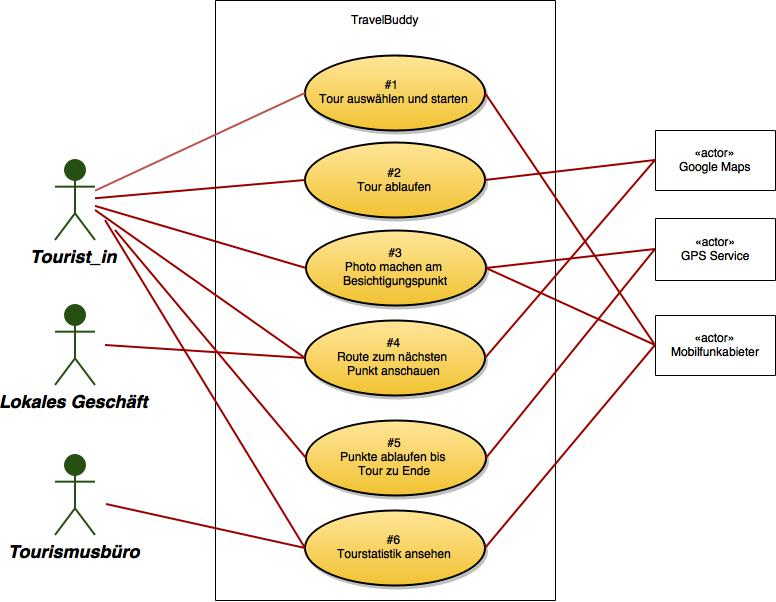
\includegraphics{Anwendungsfalldiagramm}
  \caption{Anwendungsfalldiagramm}
\end{figure}
